\documentclass[12pt]{article}

% -------------------- Packages --------------------
\usepackage{hyperref}
\usepackage{listings}
\usepackage[margin=1in]{geometry}
\usepackage{enumitem}
\usepackage{array}
\usepackage{titlesec}
\usepackage{helvet}
\renewcommand{\familydefault}{\sfdefault}

% Math packages
\usepackage{amsmath}     % For math equations
\usepackage{amssymb}     % For advanced math symbols
\usepackage{amsfonts}    % For math fonts
\usepackage{gvv}         % Custom matrix/vector formatting
\usepackage{esint}

% Other packages
\usepackage[utf8]{inputenc}
\usepackage{graphicx}
\usepackage{pgfplots}
\pgfplotsset{compat=1.18}
\usepackage{multirow}
\usepackage{float}
\usepackage{caption}
\usepackage{multicol}

% -------------------- Formatting --------------------
\titleformat{\section}{\bfseries\large}{\thesection.}{1em}{}
\setlength{\parindent}{0pt}
\setlength{\parskip}{6pt}
\renewcommand{\labelenumi}{\alph{enumi})}

% -------------------- Document --------------------
\begin{document}

\newpage
\begin{center}
\textbf{\Large AI25BTECH11034 - SUJAL CHAUHAN }\\
\textbf{2.10.23}
\end{center}

\textbf{Question:}\\
The vector(s) which is/are coplanar with the vectors $\hat{i}+\hat{j}+2\hat{k}$ and $\hat{i}+2\hat{j}+\hat{k}$, and perpendicular to vector $\hat{i}+\hat{j}+\hat{k}$ is/are.
\begin{enumerate}
    \item $\hat{\mathbf{j}} - \hat{\mathbf{k}}$
    \item $\hat{\mathbf{i}} + \hat{\mathbf{j}}$
    \item $\hat{\mathbf{i}} - \hat{\mathbf{j}}$
    \item $\hat{\mathbf{j}} + \hat{\mathbf{k}}$
\end{enumerate}

\begin{center}
\begin{tabular}{|c|c|}
\hline
Variable & Vector \\ \hline
$\vec{A}$ & $\myvec{1 \\ 1 \\ 2}$ \\ \hline
$\vec{B}$ & $\myvec{1 \\ 2 \\ 1}$ \\ \hline
$\vec{C}$ & $\myvec{1 \\ 1 \\ 1}$ \\ \hline
\end{tabular}
\end{center}

Listing options as vectors $\vec{D_i}$:

\begin{center}
\begin{tabular}{|c|c|}
\hline
Input & Vector \\ \hline
$\vec{D_1}$ & $\myvec{0 \\ 1 \\ -1}$ \\ \hline
$\vec{D_2}$ & $\myvec{1 \\ 1 \\ 1}$ \\ \hline
$\vec{D_3}$ & $\myvec{1 \\ -1 \\ 0}$ \\ \hline
$\vec{D_4}$ & $\myvec{0 \\ 1 \\ 1}$ \\ \hline
\end{tabular}
\end{center}

\newpage

\textbf{\large Checking conditions} \\[1cm]
Let equation of plane be given by:
\begin{align}
    \vec{n}^\top\vec{X}=1
\end{align}
Let's find general solution $\vec{n}$ which is perpendicular to the plane 
\begin{align}
    \myvec{A && B}^\top\vec{n}=\myvec{1 \\ 1}
\end{align}
\begin{align}
&\text{Given:} \quad
  \myvec{1 & 1 & 2\\ 1 & 2 & 1}\vec{n} = \myvec{1 \\ 1} \\[1em]
\end{align}
\begin{align}
&\text{We want to solve:} \quad 
\myvec{1 & 1 & 2 \\ 1 & 2 & 1}\vec{n} = \myvec{1 \\ 1}, 
\quad \vec{n} = \myvec{n_1 \\ n_2 \\ n_3} \\[1em]
%
&\text{Form the augmented matrix:} \nonumber \\[0.5em]
&\myvec{1 & 1 & 2 & \vline & 1 \\ 1 & 2 & 1 & \vline & 1} \\[1em]
%
&\xrightarrow{R_2 \to R_2 - R_1}
\myvec{1 & 1 & 2 & \vline & 1 \\ 0 & 1 & -1 & \vline & 0} \\[1em]
%
&\xrightarrow{R_1 \to R_1 - R_2}
\myvec{1 & 0 & 3 & \vline & 1 \\ 0 & 1 & -1 & \vline & 0} \\[1em]
%
&\text{Thus the equations are:} \nonumber \\[0.5em]
&n_1 + 3n_3 = 1, \quad n_2 - n_3 = 0 \\[1em]
%
&\text{Let } n_3 = a \in \mathbb{R}, \quad
n_2 = a, \quad n_1 = 1 - 3a \\[1em]
%
&\text{So the general solution is:} \nonumber \\[0.5em]
&\vec{n} = \myvec{1 - 3a \\ a \\ a}, \quad a \in \mathbb{R}
\end{align}


General solution is 
\begin{align}
\vec{n} = \myvec{1 - 3a\\ a \\ a}
\end{align}


Now any vector following both condition will be solution of the equation:
\begin{align}
    \myvec{ n & C}^\top\vec{D_i}=\myvec{0\\0}
\end{align}
Checking Values for all options:
\begin{align}
    \myvec{1-3a & a & a \\ 1 & 1 &1}\vec{D_i}=\myvec{0 \\ 0}
\end{align}
\begin{center}
\begin{tabular}{|c|c|c|}
\hline
Vector & $ \myvec{1-3a & a & a \\ 1 & 1 &1}\vec{D_i}$ & Satisfies\\ \hline
$\vec{D_1}$ & $\myvec{0\\0}$ & Yes \\ \hline
$\vec{D_2}$ & $\myvec{1-2a\\2}$  & No  \\ \hline
$\vec{D_3}$ & $\myvec{1-4a\\0}$ & No \\ \hline
$\vec{D_4}$ & $\myvec{2a\\2}$  & No  \\ \hline
\end{tabular}
\end{center}

So only $\vec{D_1}$ satisfies both conditions.

\newpage
\begin{figure}[H]
    \centering
    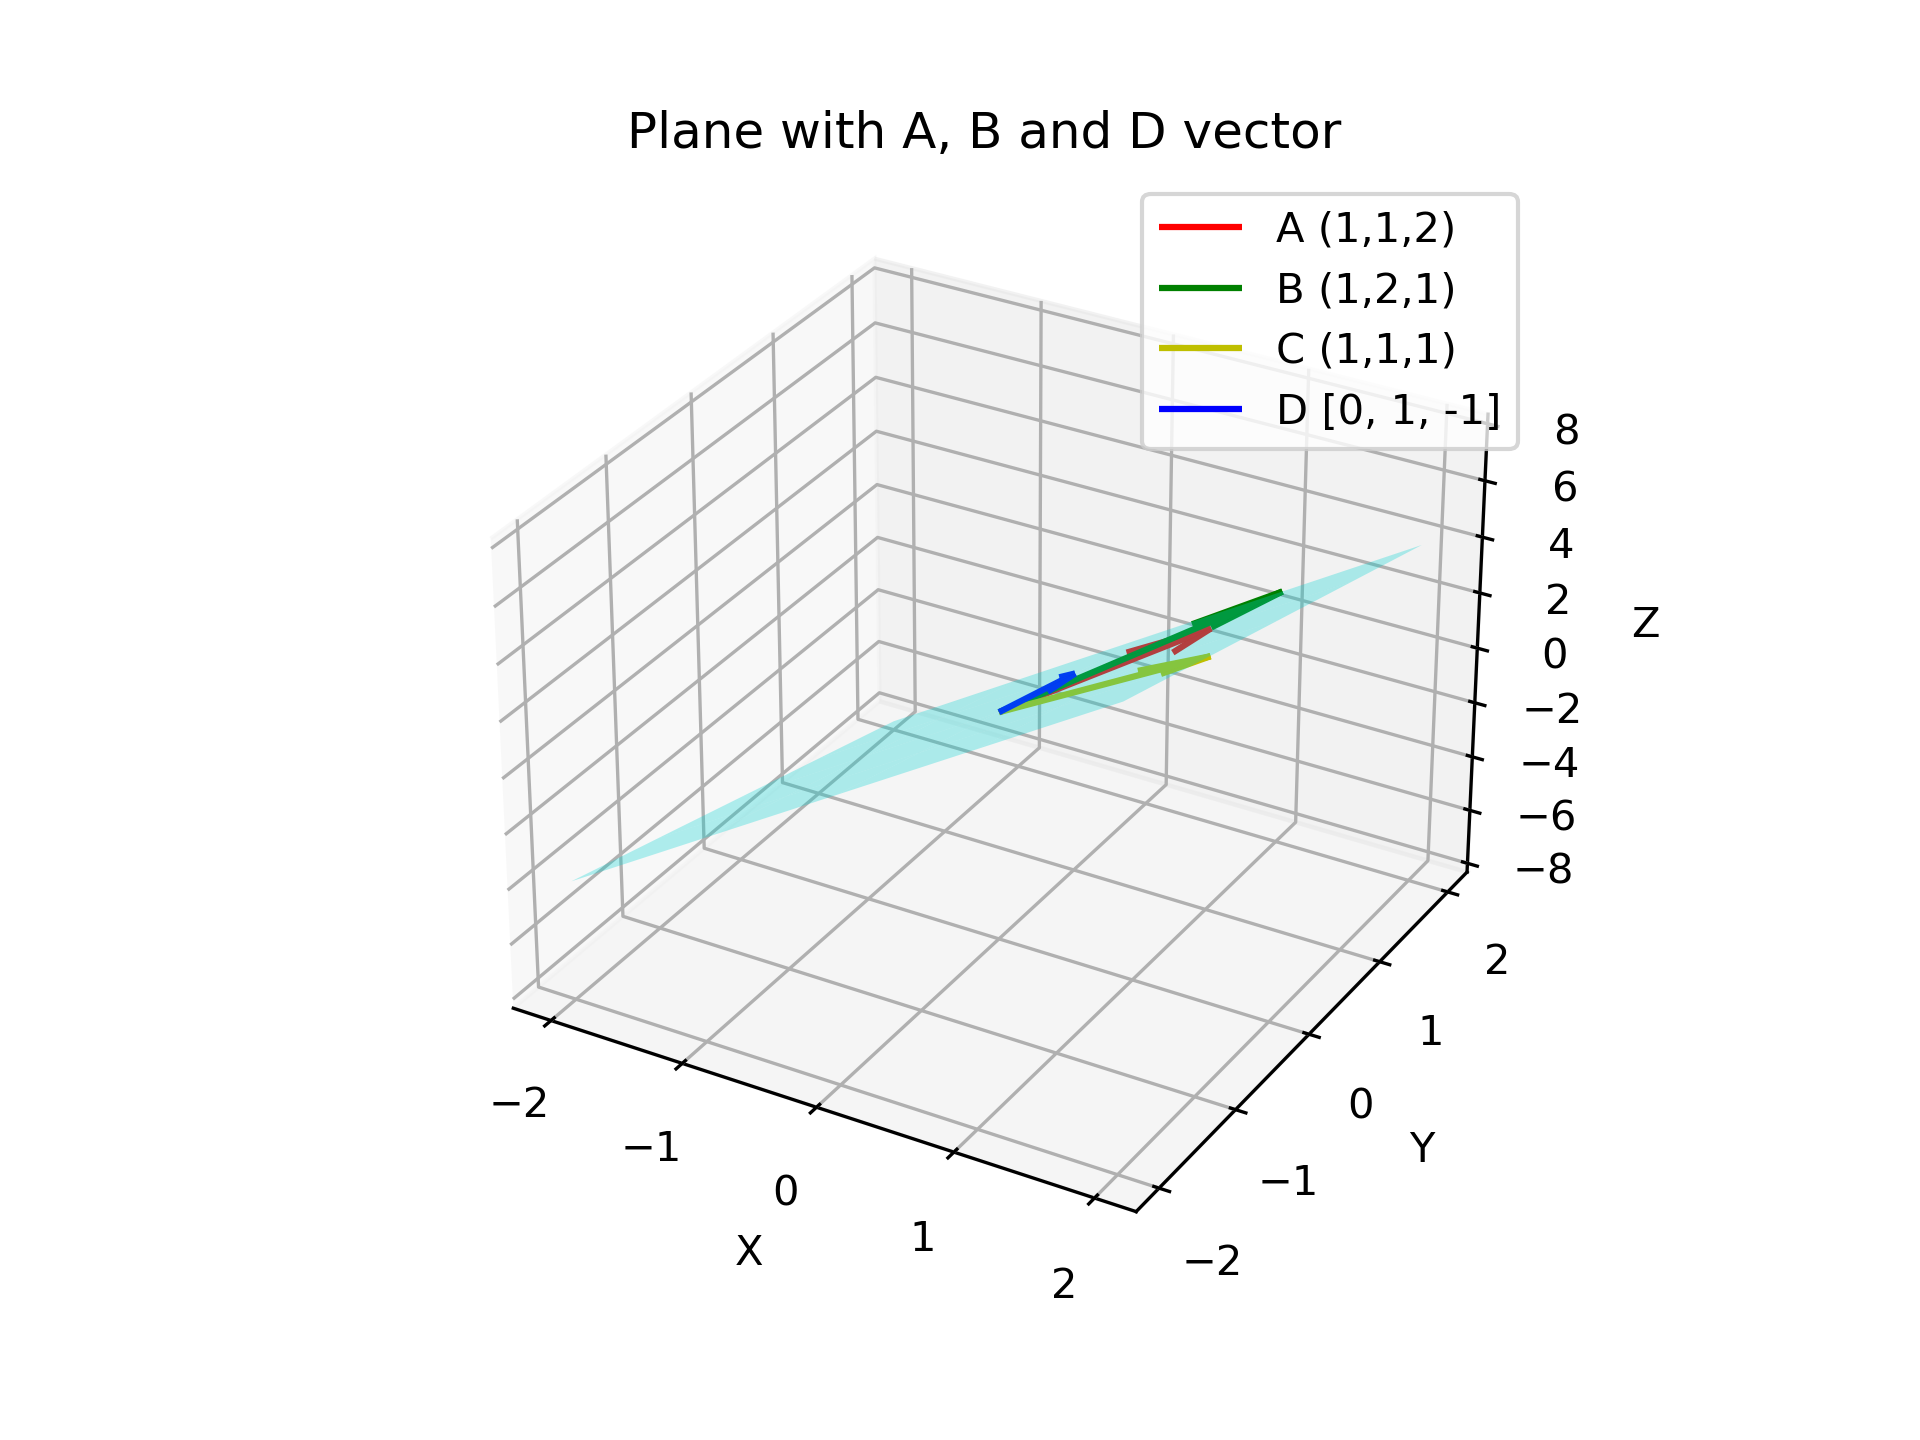
\includegraphics[width=0.6\linewidth]{figures/plane_1.png}
    \caption{Vector $\vec{D_1}$ in plane}
\end{figure}

\begin{figure}[H]
    \centering
    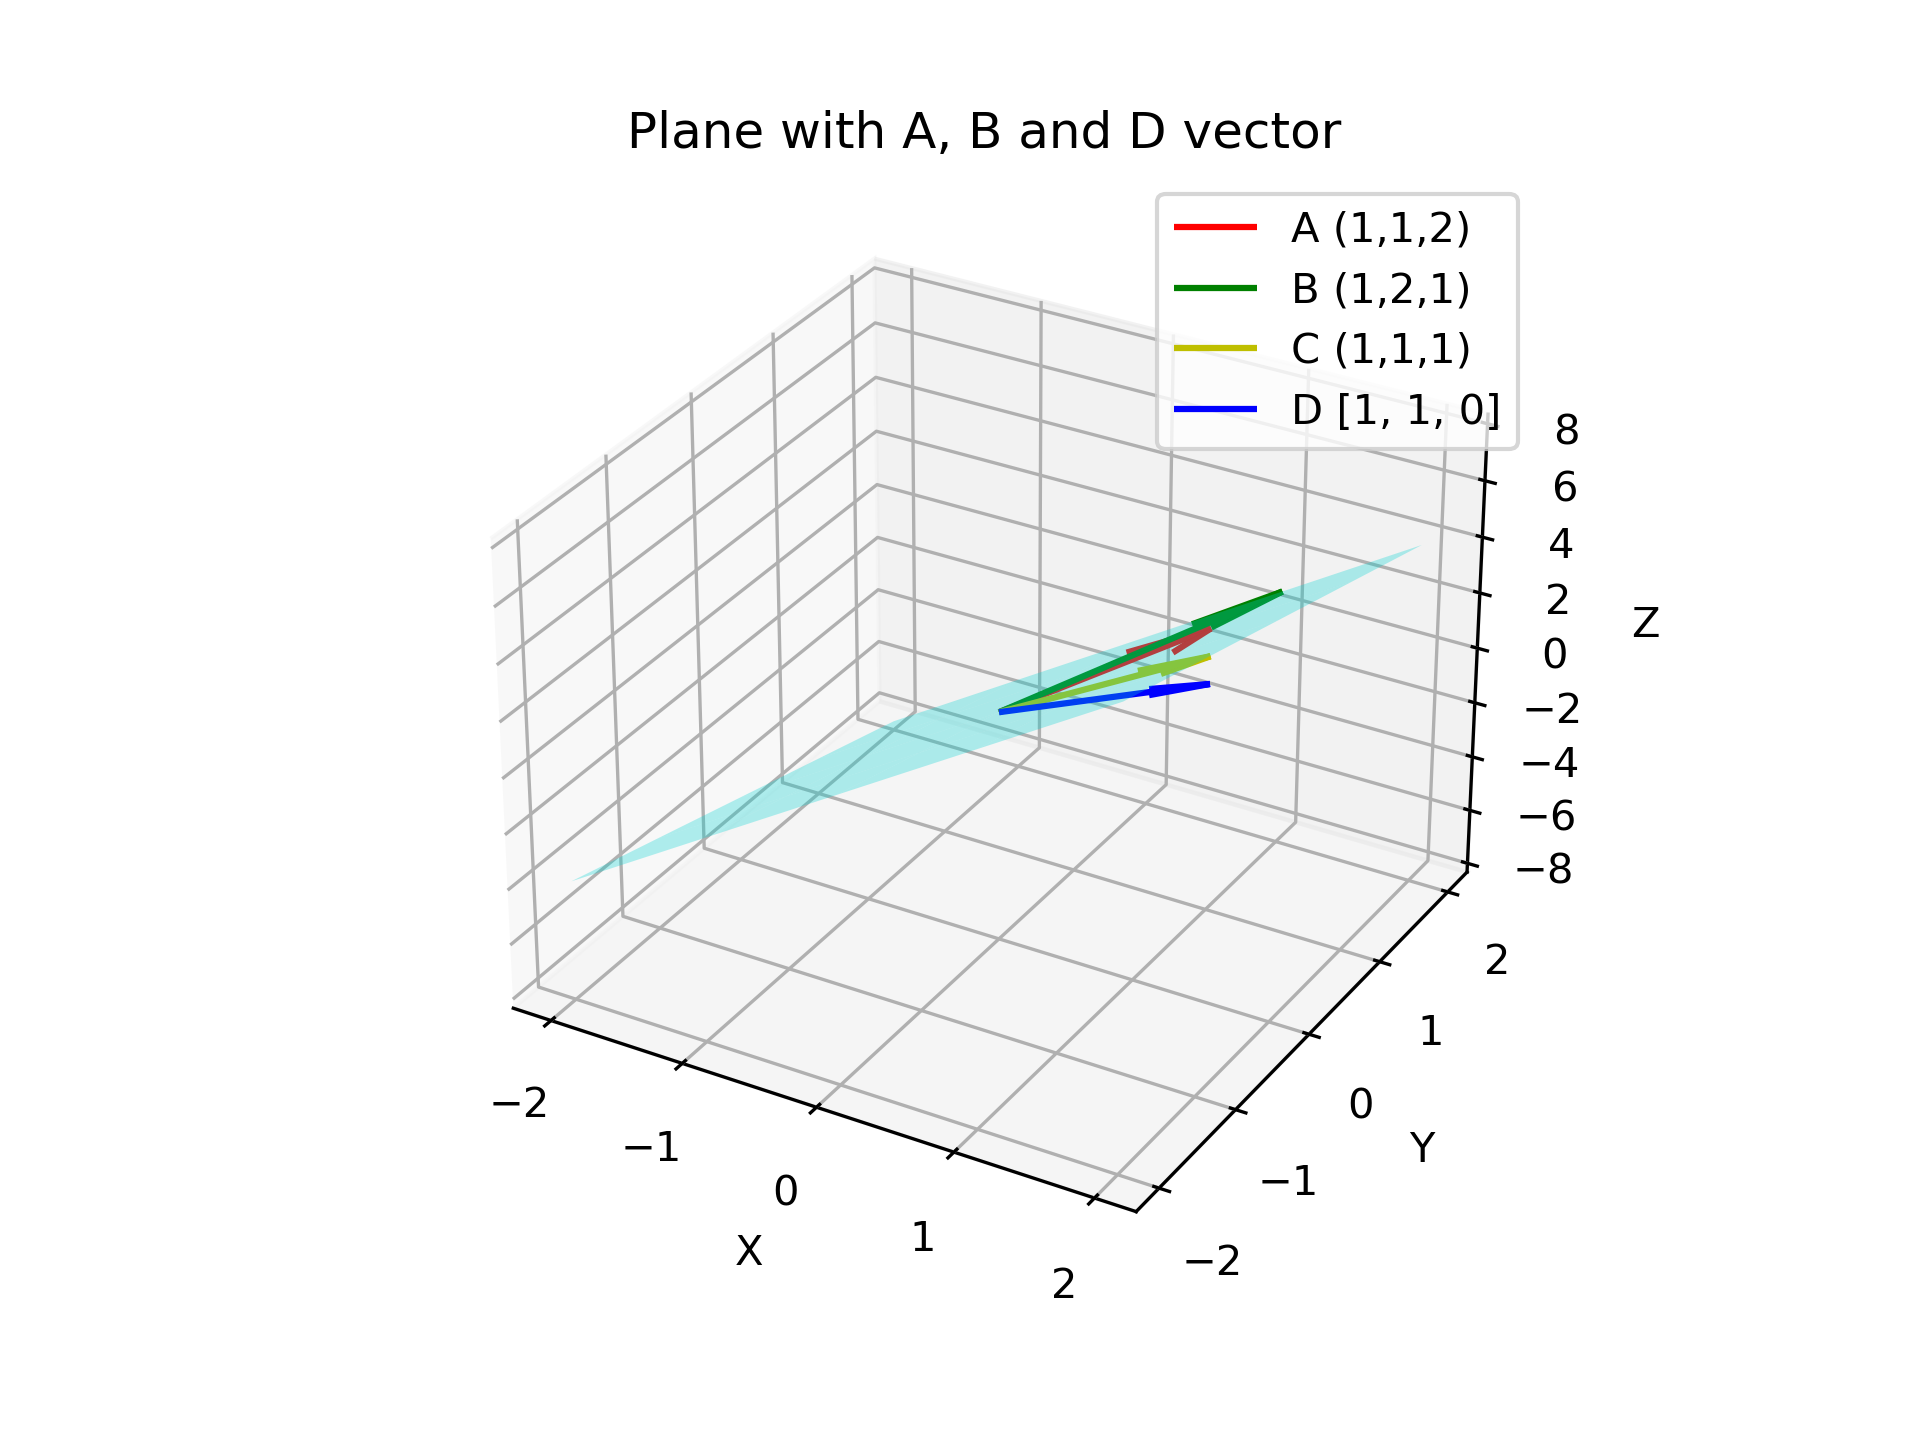
\includegraphics[width=0.6\linewidth]{figures/plane_2.png}
    \caption{Vector $\vec{D_2}$ not coplanar}
\end{figure}

\begin{figure}[H]
    \centering
    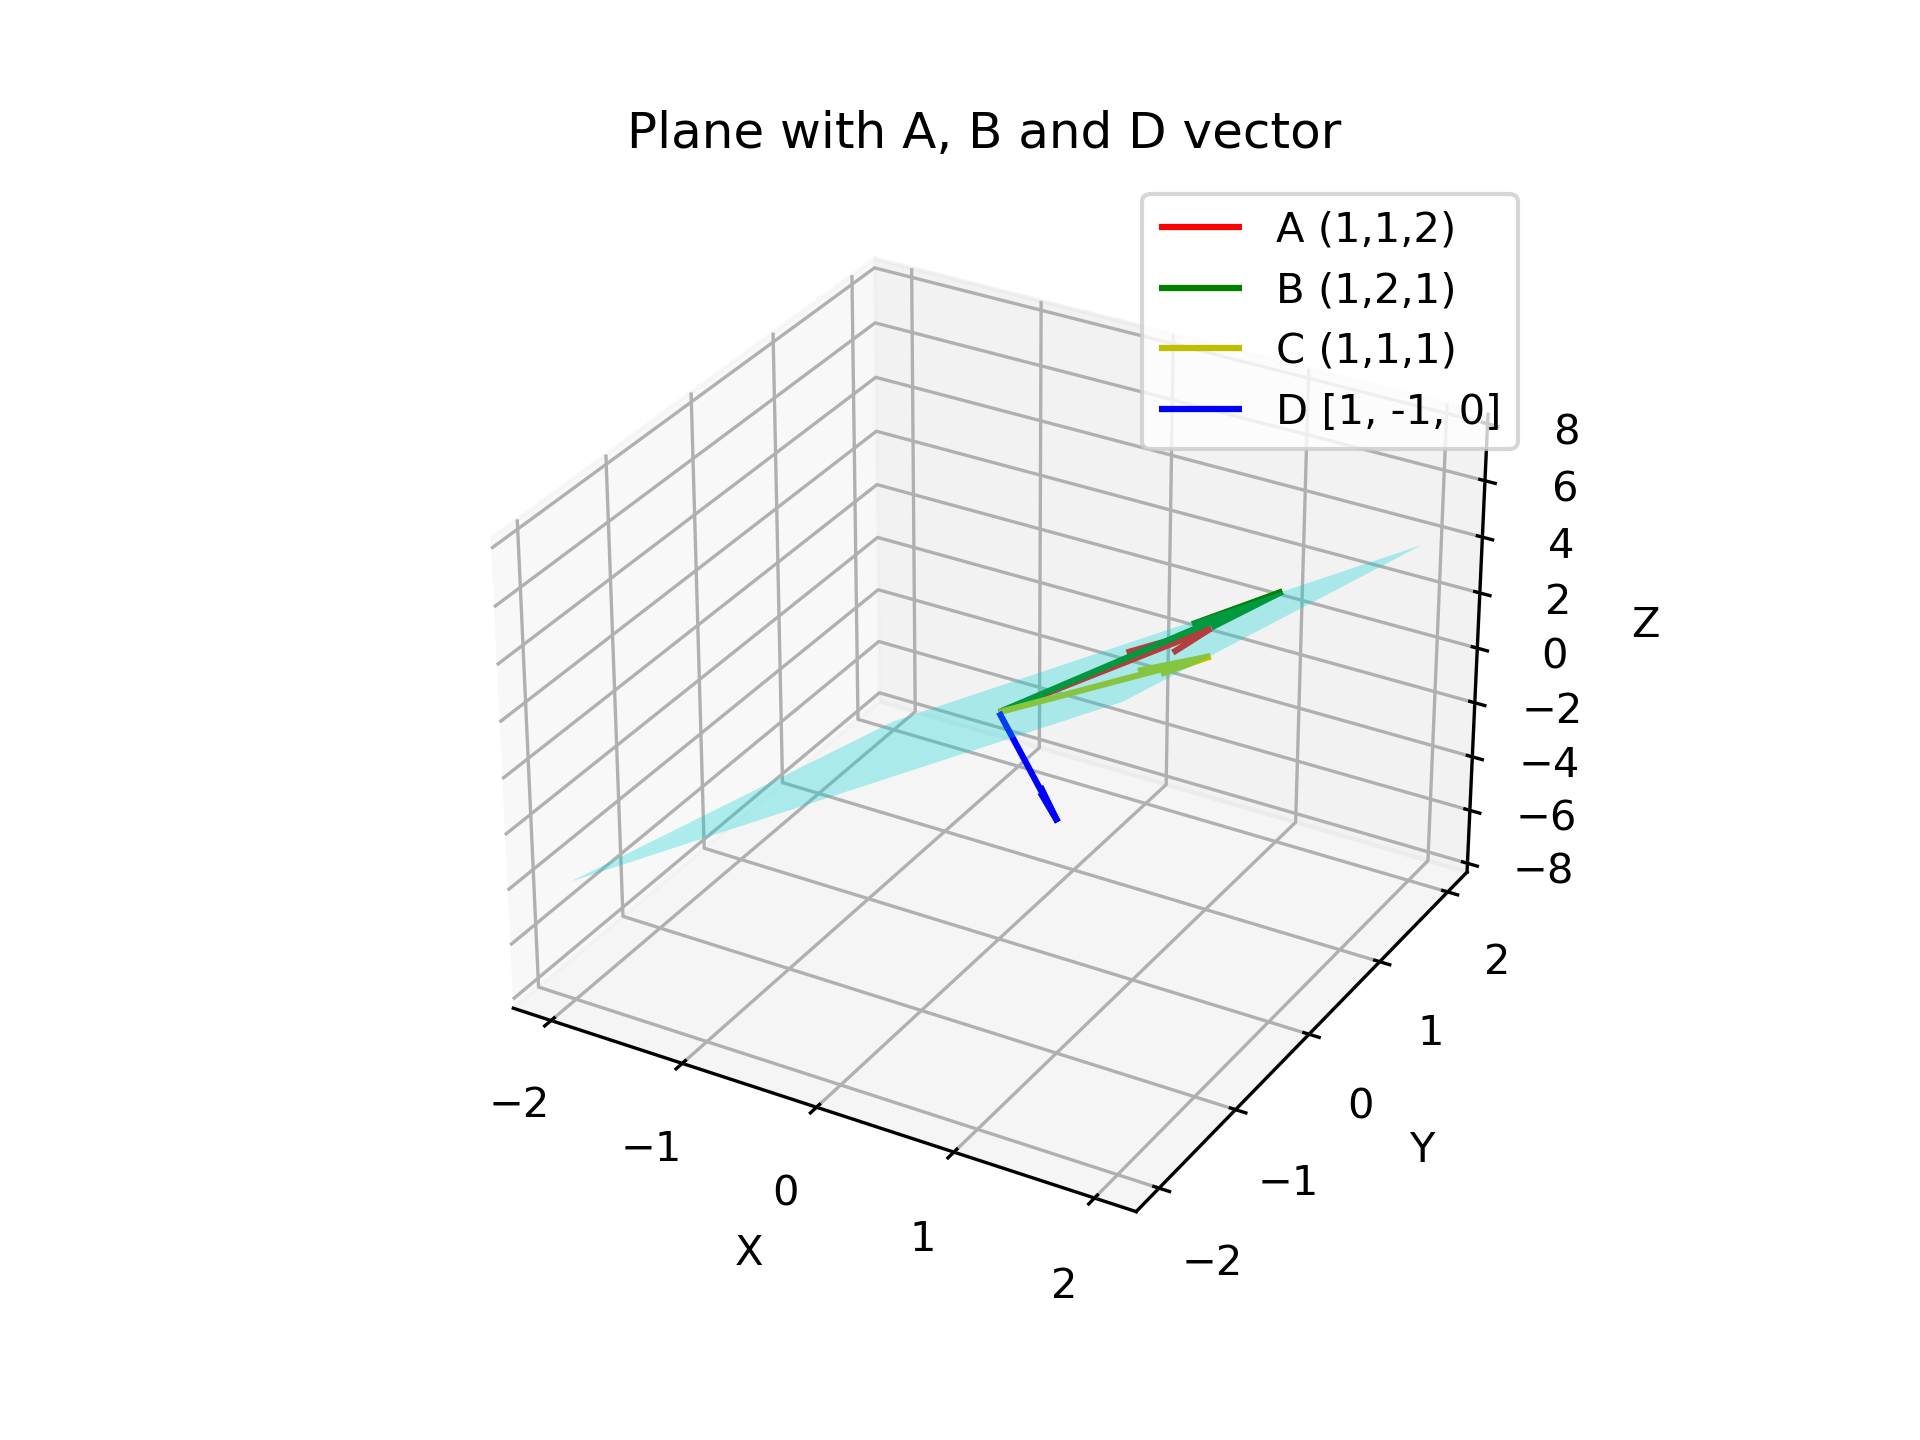
\includegraphics[width=0.6\linewidth]{figures/plane_3.png}
    \caption{Vector $\vec{D_3}$ not coplanar}
\end{figure}

\begin{figure}[H]
    \centering
    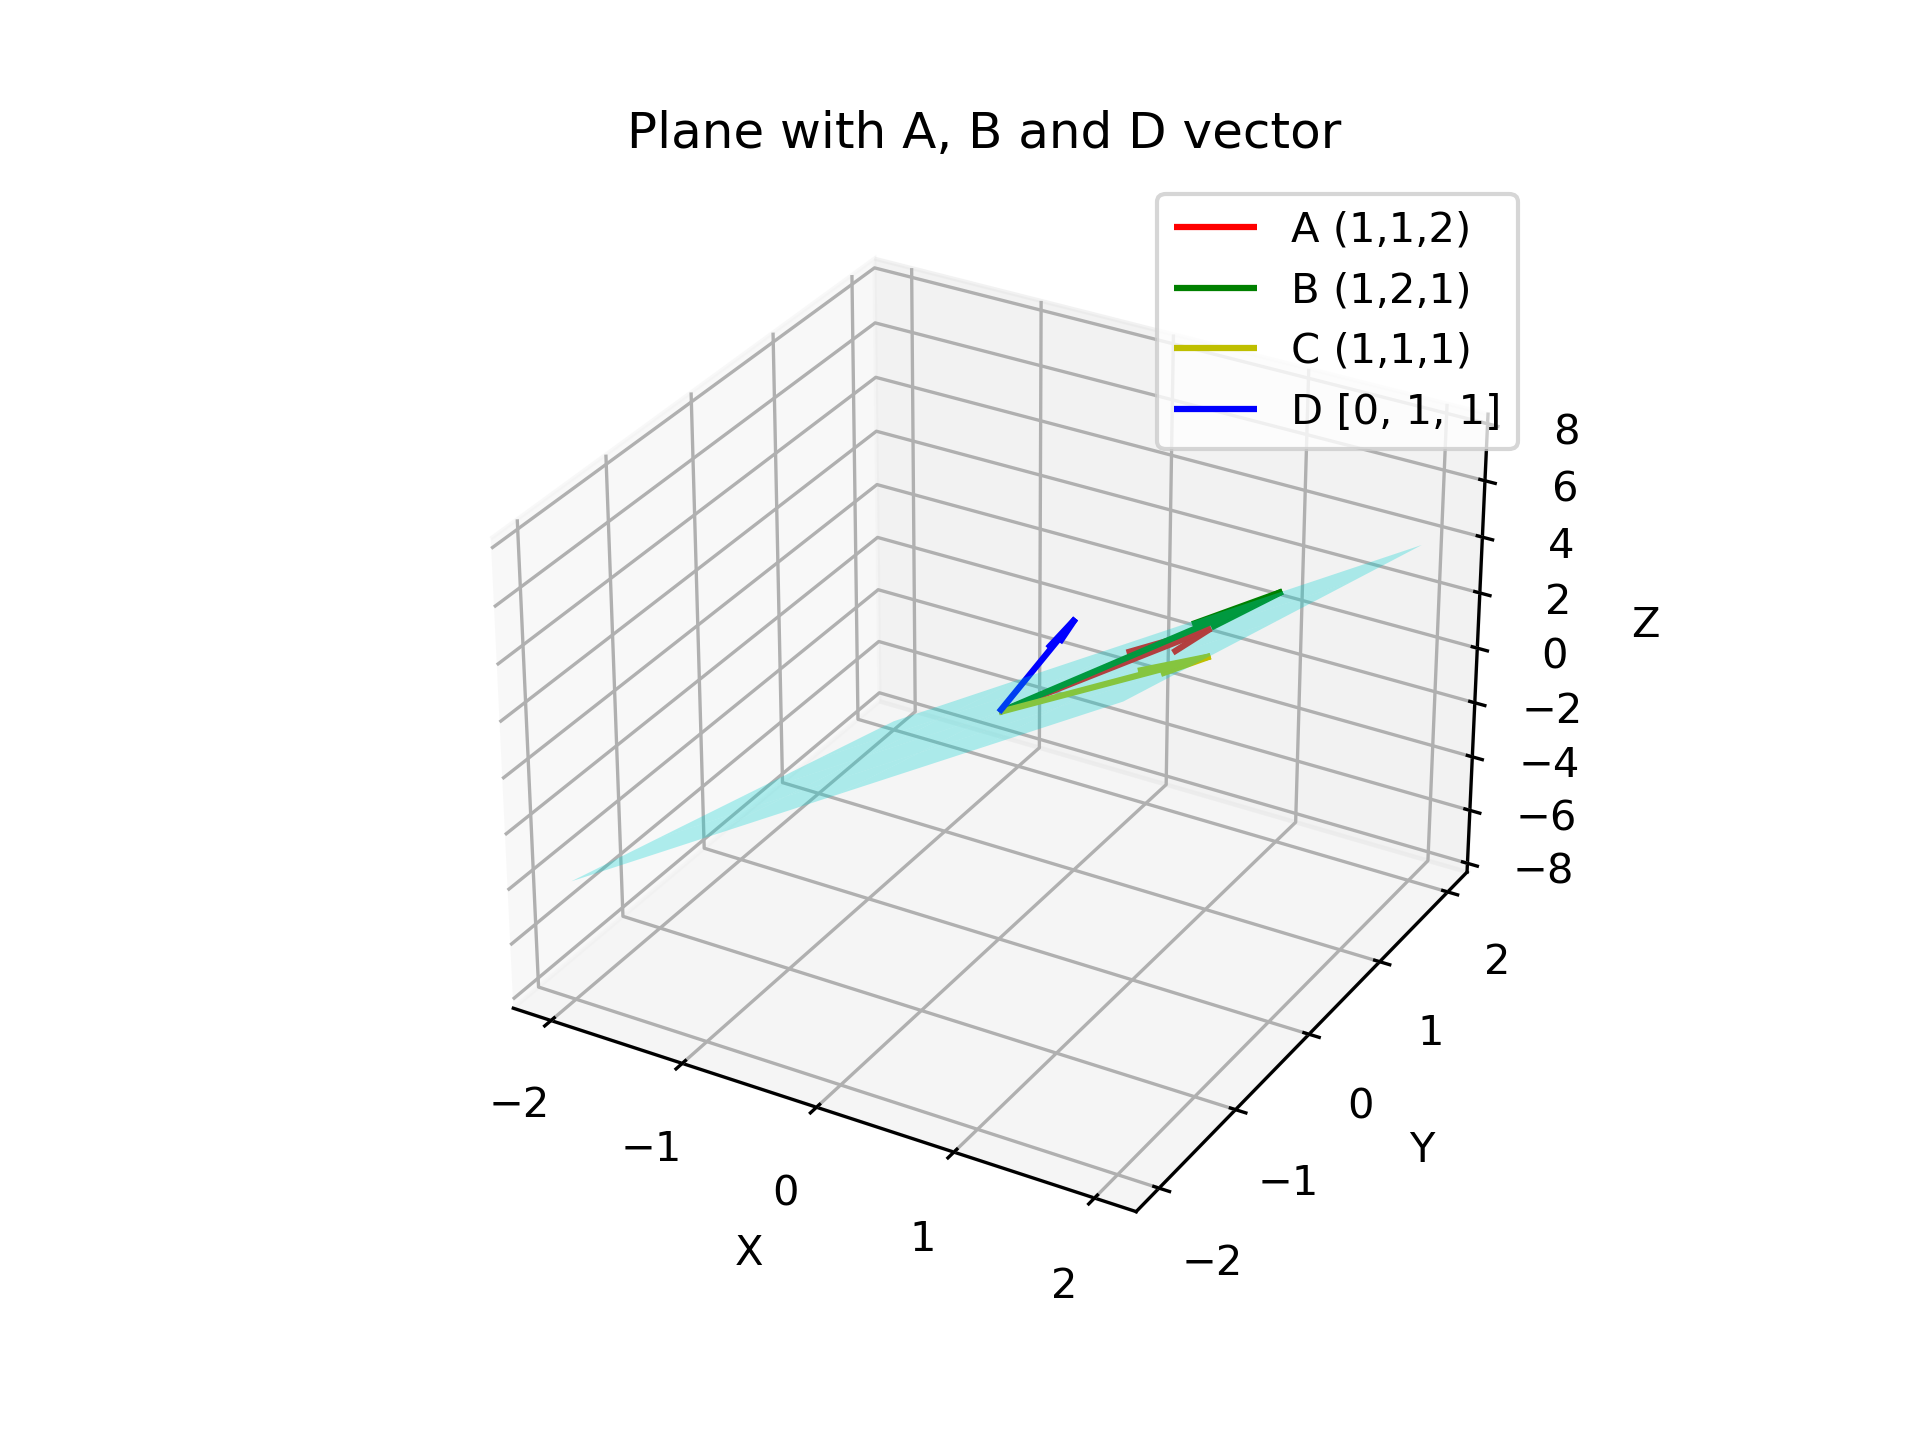
\includegraphics[width=0.6\linewidth]{figures/plane_4.png}
    \caption{Vector $\vec{D_4}$ not coplanar}
\end{figure}

\end{document}

